\documentclass[12pt, a4paper, oneside]{Thesis} % Paper size, default font size and one-sided paper
\usepackage{wrapfig}
\usepackage{lscape}
\usepackage{rotating}
\usepackage{graphicx}
\usepackage{caption}
\usepackage{amsmath}


\usepackage{lineno,hyperref}
\modulolinenumbers[5]


\usepackage{amssymb}
\usepackage{graphicx}
\usepackage{array}
\usepackage{float}
\usepackage{placeins}
\usepackage{stackengine}
\usepackage{url}
\usepackage{numprint}
\usepackage{caption}

\usepackage{booktabs}  
\usepackage{siunitx}
%\usepackage[showframe=false]{geometry}
\usepackage{subfigure}

\nprounddigits{3}
\newcolumntype{P}[1]{>{\centering\arraybackslash}p{#1}}
\newcolumntype{M}[1]{>{\centering\arraybackslash}m{#1}}

\setstackEOL{\#}
\setstackgap{L}{12pt}


%\usepackage{subcaption} %incompatible with subfig
\graphicspath{{Pictures/}} % Specifies the directory where pictures are stored
\usepackage{natbib} % Use the natbib reference package - read up on this to edit the reference style; if you want text (e.g. Smith et al., 2012) for the in-text references (instead of numbers), remove 'numbers' v


\hypersetup{urlcolor=black, colorlinks=false} % Colors hyperlinks in blue - change to black if annoyingv`	

\thesistitle{Vision-Augmented Motion Forecasting: An Investigation into the Integration of BEV Features with AgentFormer}
\supervisor{Debaditya Roy}
\degree{Bachelor of Technology + Master of Technology}
\degreemajor{Computer Science and Engineering}
\authors{K. Tharun Selvam}
\rollno{22CS30033}
\university{Indian Institute of Technology Kharagpur}
\department{Department of Computer Science and Engineering}
\unisite{http://www.iitkgp.ac.in}
\depsite{http://www.iitkgp.ac.in/department/CE}
\placeshrt{Kharagpur}
\placelng{Kharagpur - 721302, India}
\datesub{30th October 2025}
\datesig{30th October 2025}
\semsub{Autumn Semester, 2016-17}
\keywords{Motion Forecasting, Autonomous Driving, Multi-modal Fusion, Bird's-Eye-View, Deep Learning}
\coursecd{Project-I (CE57006) }

\title{\ttitle} % Defines the thesis title - don't touch this
\begin{document}
%\makeatletter
%\renewcommand*{\NAT@nmfmt}[1]{\textsc{#1}}
%\makeatother

% prints author names as small caps


\frontmatter % Use roman page numbering style (i, ii, iii, iv...) for the pre-content pages

\setstretch{1.6} % Line spacing of 1.6 (double line spacing)

% Define the page headers using the FancyHdr package and set up for one-sided printing
\fancyhead{} % Clears all page headers and footers
\rhead{\thepage} % Sets the right side header to show the page number
\lhead{} % Clears the left side page header

%\pagestyle{fancy} % Finally, use the "fancy" page style to implement the FancyHdr headers

\newcommand{\HRule}{\rule{\linewidth}{0.5mm}} % New command to make the lines in the title page

% PDF meta-data
\hypersetup{pdftitle={\ttitle}}
\hypersetup{pdfsubject=\subjectname}
\hypersetup{pdfauthor=\authornames}
\hypersetup{pdfkeywords=\keywordnames}

%----------------------------------------------------------------------------------------
%	TITLE PAGE
%----------------------------------------------------------------------------------------
\maketitle
%\titlepg % Add a gap in the Contents, for aesthetics

\clearpage % Start a new page

%----------------------------------------------------------------------------------------
%	DECLARATION PAGE
%	Your institution may give you a different text to place here
%----------------------------------------------------------------------------------------


\Declaration% Add a gap in the Contents, for aesthetics


%----------------------------------------------------------------------------------------
%\tCERTIFICATE PAGE
%----------------------------------------------------------------------------------------

\addtotoc{Certificate} % Add the "Abstract" page entry to the Contents

\certificate{\addtocontents{toc}{} % Add a gap in the Contents, for aesthetics

\clearpage % Start a new page

%----------------------------------------------------------------------------------------
%\tABSTRACT PAGE
%----------------------------------------------------------------------------------------

\addtotoc{Abstract} % Add the "Abstract" page entry to the Contents

\abstract{\addtocontents{toc}{} % Add a gap in the Contents, for aesthetics

This thesis investigates the integration of Bird's-Eye-View (BEV) features, generated by the BEVDepth model, into the AgentFormer motion forecasting framework. The initial hypothesis was that the rich visual context provided by BEV features would enhance AgentFormer's prediction accuracy. However, experimental results showed a degradation in performance. This work details the methodology of the integration, analyzes the potential reasons for the negative results, and proposes future research directions to better leverage visual information in motion forecasting models.
}

\clearpage % Start a new page



%----------------------------------------------------------------------------------------
%\tLIST OF CONTENTS/FIGURES/TABLES PAGES
%----------------------------------------------------------------------------------------

\pagestyle{fancy} % The page style headers have been "empty" all this time, now use the "fancy" headers as defined before to bring them back

\lhead{\emph{Contents}} % Set the left side page header to "Contents"
\tableofcontents % Write out the Table of Contents

\lhead{\emph{List of Figures}} % Set the left side page header to "List of Figures"
\listoffigures % Write out the List of Figures

\lhead{\emph{List of Tables}} % Set the left side page header to "List of Tables"
\listoftables % Write out the List of Tables

%----------------------------------------------------------------------------------------
%\tTHESIS CONTENT - CHAPTERS
%----------------------------------------------------------------------------------------

\mainmatter % Begin numeric (1,2,3...) page numbering

\pagestyle{fancy} % Return the page headers back to the "fancy" style

% Include the chapters of the thesis as separate files from the Chapters folder
% Uncomment the lines as you write the chapters

% Chapter Template

\chapter{Introduction} % Main chapter title

\label{Chapter1} % Change X to a consecutive number; for referencing this chapter elsewhere, use \ref{ChapterX}

\lhead{Chapter 1. \emph{Introduction}} % Change X to a consecutive number; this is for the header on each page - perhaps a shortened title

%----------------------------------------------------------------------------------------
%\tSECTION 1
%---------------------------------------------------------------------------------------
\section{Introduction and Motivation}

\subsection{The Big Picture}

The pursuit of fully autonomous driving has become one of the most significant and challenging endeavors in modern engineering. A critical component of any autonomous system is the ability to perceive its environment and anticipate the future actions of other agents. Accurate and reliable motion forecasting is paramount for ensuring the safety and efficiency of autonomous vehicles. By predicting the future trajectories of surrounding vehicles, pedestrians, and cyclists, an autonomous car can make informed decisions, plan safe paths, and avoid potential collisions.

\subsection{Problem Definition}

Multi-agent motion forecasting in dynamic and interactive environments is a complex problem. The future trajectory of an agent is not only influenced by its own past motion but also by its interactions with other agents and its understanding of the surrounding scene. A robust motion forecasting system must be able to model these complex dependencies to generate accurate and socially compliant predictions. The challenges are manifold, including but not limited to:

\begin{itemize}
    \item Modeling the interactions between multiple agents.
    \item Incorporating scene context, such as lane geometry, traffic lights, and static obstacles.
    \item Handling the inherent uncertainty and multi-modality of future movements.
\end{itemize}

\subsection{The Motivation}

To address these challenges, recent research has focused on developing deep learning models that can learn complex patterns from large-scale datasets. AgentFormer is a state-of-the-art motion forecasting model that has demonstrated excellent performance in modeling agent interactions using a transformer-based architecture. However, AgentFormer primarily relies on trajectory information and has a limited understanding of the rich visual context of the scene.

On the other hand, Bird's-Eye-View (BEV) representations have emerged as a powerful way to represent the 3D world for autonomous driving tasks. BEVDepth is a model that can generate dense and detailed BEV feature maps from multiple camera images, capturing the geometry and semantics of the scene. The central hypothesis of this thesis is that by integrating the rich visual context from BEVDepth into the AgentFormer model, we can improve its motion forecasting accuracy.

This work explores the integration of these two powerful models. The motivation is to provide AgentFormer with a more comprehensive understanding of the scene, enabling it to make more informed predictions. We hypothesized that the BEV features would provide crucial information about lane boundaries, crosswalks, traffic lights, and other static and dynamic elements of the scene that are not available from trajectory data alone.

However, the results of our experiments were surprising. The integration of BEV features, contrary to our initial hypothesis, led to a degradation in the performance of the AgentFormer model. This thesis will detail the methodology of the integration, present the results, and, most importantly, provide a thorough analysis of the potential reasons for this unexpected outcome. By investigating why the integration failed, we aim to provide valuable insights for future research on multi-modal fusion in motion forecasting.
% Chapter Template

\chapter{Literature Review} % Main chapter title

\label{Chapter2} % Change X to a consecutive number; for referencing this chapter elsewhere, use \ref{ChapterX}

\lhead{Chapter 2. \emph{Literature Review}} % Change X to a consecutive number; this is for the header on each page - perhaps a shortened title

%----------------------------------------------------------------------------------------
%\t\tSECTION 1
%---------------------------------------------------------------------------------------
\section{Motion Forecasting}

Motion forecasting has been a long-standing problem in robotics and autonomous driving. Early approaches relied on physics-based models, such as the constant velocity and constant acceleration models. While simple and efficient, these models fail to capture the complex and interactive nature of real-world traffic scenarios.

With the advent of machine learning, classical methods like Kalman filters, Hidden Markov Models (HMMs), and Gaussian Processes were employed to model the uncertainty and dynamics of motion. However, these models often struggle with the high dimensionality and non-linearity of multi-agent systems.

In recent years, deep learning has become the dominant paradigm for motion forecasting \citep{Shi2025MotionFF}. Recurrent Neural Networks (RNNs), particularly Long Short-Term Memory (LSTM) networks, have been widely used to model the sequential nature of trajectory data. Convolutional Neural Networks (CNNs) have also been used to extract features from rasterized scene images. More recently, attention mechanisms have been introduced to better capture the complex dependencies in motion data \citep{Mao2021Multi-levelMA, Ding2022DeepLW}.

\section{Agent-Centric vs. Scene-Centric Approaches}

Modern deep learning-based motion forecasting models can be broadly categorized into two paradigms: agent-centric and scene-centric.

\textbf{Agent-centric} approaches model the trajectory of each agent independently, often using RNNs to encode the past motion and decode the future. These models are computationally efficient but often fail to capture the complex interactions between agents.

\textbf{Scene-centric} approaches, on the other hand, process all agents in a scene simultaneously, often using a shared architecture like a CNN or a graph neural network. These models are better at capturing interactions but can be computationally expensive and may struggle with a large number of agents.

\section{AgentFormer}

AgentFormer \citep{yuan2021agentformer} is a transformer-based architecture designed for multi-agent trajectory forecasting. It addresses the limitations of previous methods that model the temporal (time) and social (agent interactions) dimensions of trajectories separately. The key innovation of AgentFormer is its ability to model these two dimensions simultaneously, allowing for a more holistic understanding of the scene dynamics.

\subsection{Simultaneous Socio-Temporal Modeling}

Unlike traditional approaches that first encode temporal information for each agent and then model social interactions (or vice-versa), AgentFormer processes a flattened sequence of all agents' trajectories across all timesteps. This allows the model to learn direct relationships between an agent's state at one time and another agent's state at a future time.

\subsection{Agent-Aware Attention}

A core contribution of AgentFormer is the novel \textbf{agent-aware attention} mechanism. Standard attention mechanisms in transformers do not distinguish between different agents in a sequence. To overcome this, AgentFormer uses two sets of queries and keys: one for \textbf{intra-agent attention} (an agent attending to its own past states) and another for \textbf{inter-agent attention} (an agent attending to the states of other agents). This is achieved through a masking mechanism that identifies whether a query and a key belong to the same agent. This allows the model to learn different patterns for an agent's own motion and its interaction with others.

\subsection{CVAE-based Probabilistic Forecasting}

To model the inherent uncertainty and multi-modality of future trajectories, AgentFormer is built upon a Conditional Variational Autoencoder (CVAE) framework. It introduces a latent variable for each agent to represent its "intent." The model learns a joint distribution over the latent intents of all agents, enabling it to generate socially-aware and diverse future trajectories. The CVAE framework consists of:

\begin{itemize}
    \item \textbf{Past Encoder:} An AgentFormer encoder that processes the past trajectories of all agents to produce a context representation.
    \item \textbf{Future Encoder:} An AgentFormer decoder that processes the ground truth future trajectories (during training) to infer the posterior distribution of the latent variables.
    \item \textbf{Future Decoder:} An autoregressive AgentFormer decoder that takes the context representation and a sampled latent code to generate the future trajectory one step at a time.
\end{itemize}

\begin{figure}[h]
\centering
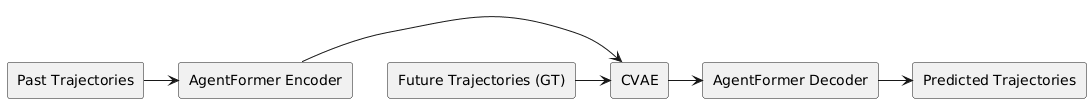
\includegraphics[width=\textwidth]{agentformer_architecture.png}
\caption{Overview of the AgentFormer-based multi-agent trajectory prediction framework. Figure from \citep{yuan2021agentformer}.}
\label{fig:agentformer_architecture}
\end{figure}


\section{Bird's-Eye-View (BEV) Representations}

Bird's-Eye-View (BEV) is a popular representation for scene understanding in autonomous driving. It provides a top-down view of the 3D world, which is a natural and intuitive representation for tasks like object detection, segmentation, and motion planning.

BEV representations have several advantages over other representations, such as camera-view or point cloud representations:

\begin{itemize}
    \item They provide a unified representation of the scene, where objects are represented at their correct metric scale and location.
    \item They are invariant to camera perspective changes.
    \item They are well-suited for downstream tasks like planning and control.
\end{itemize}

\section{BEVDepth}

BEVDepth \citep{li2022bevdepth} is a leading model for generating dense BEV feature maps from multiple camera images. It addresses the challenge of accurately projecting image features into the 3D world by explicitly predicting the depth of each pixel in the image.

The BEVDepth model consists of several key components:

\begin{itemize}
    \item A camera-view encoder that extracts features from each camera image.
    \item A depth prediction network that estimates the depth of each pixel.
    \item A view transformer that lifts the 2D image features into a 3D point cloud using the predicted depth.
    \item A voxel pooling layer that aggregates the 3D points into a dense BEV feature map.
\end{itemize}

BEVDepth has achieved state-of-the-art performance on several BEV segmentation and detection benchmarks. Its ability to generate high-quality BEV features makes it an attractive candidate for providing visual context to motion forecasting models.

\section{Gap in the Literature}

While both AgentFormer and BEVDepth are powerful models in their respective domains, their integration has not been thoroughly explored. AgentFormer excels at modeling agent interactions but lacks a deep understanding of the visual scene. BEVDepth, on the other hand, provides a rich representation of the visual scene but does not directly perform motion forecasting.

This thesis aims to fill this gap by investigating the integration of BEVDepth with AgentFormer. The goal is to leverage the strengths of both models to create a more robust and accurate motion forecasting system. The surprising negative results of this integration, as will be discussed in the following chapters, highlight the challenges of multi-modal fusion and provide valuable insights for future research in this area.


% Chapter Template

\chapter{Dataset} % Main chapter title

\label{Chapter2_Dataset} % Change X to a consecutive number; for referencing this chapter elsewhere, use \ref{ChapterX}

\lhead{Chapter 2. \emph{Dataset}} % Change X to a consecutive number; this is for the header on each page - perhaps a shortened title

%----------------------------------------------------------------------------------------
%\tSECTION 1
%---------------------------------------------------------------------------------------
\section{nuScenes Dataset}

The nuScenes dataset \citep{caesar2020nuscenes} is a large-scale, multi-modal dataset for autonomous driving, developed by Motional (formerly nuTonomy). It was the first dataset to feature a full autonomous vehicle sensor suite, including 6 cameras, 5 radars, and 1 lidar, all with a full 360-degree field of view. This comprehensive sensor setup provides a rich and holistic view of the environment, which is crucial for developing robust perception systems.

\subsection{Sensor Suite}
The sensor setup, as detailed in Table \ref{tab:nuscenes_sensors}, is critical for our project. The BEVDepth model, which we use for scene understanding, is designed to consume images from all 6 cameras. The Lidar and Radar data provide ground-truth depth and velocity information, which, while not used as direct model inputs, are foundational to the dataset's ground-truth annotations.

\begin{table}[h]
\centering
\caption{nuScenes Sensor Specifications. (Adapted from \citep{caesar2020nuscenes})}
\label{tab:nuscenes_sensors}
\begin{tabular}{l p{9cm}}
\hline
\textbf{Sensor} & \textbf{Details} \\
\hline
6x Camera & RGB, 12Hz capture, $1600 \times 900$ resolution, 360° coverage. \\
1x Lidar & 32-beam, 20Hz capture, 360° horizontal FOV, $\le 70m$ range. \\
5x Radar & 77GHz, 13Hz capture, $\le 250m$ range, provides velocity. \\
GPS \& IMU & For localization and sensor synchronization. \\
\hline
\end{tabular}
\end{table}

\subsection{Data Collection}

The data was collected in Boston and Singapore, two cities known for their dense traffic and challenging driving scenarios. The dataset comprises 1000 scenes, each 20 seconds long. These scenes were carefully selected to include a wide variety of interesting and challenging situations, such as high traffic density, rare object classes, and complex maneuvers. The dataset is split into 700 scenes for training, 150 for validation, and 150 for testing. The dataset is also notable for its inclusion of diverse weather and lighting, with 19.4\% of scenes captured in the rain and 11.6\% at night.

\subsection{Annotations}

nuScenes provides detailed annotations for 23 object classes, including various types of vehicles, pedestrians, and cyclists. The annotations consist of 3D bounding boxes, instance masks, and 8 attributes, such as visibility, activity, and pose. With 7 times more annotations and 100 times more images than the pioneering KITTI dataset, nuScenes represents a significant leap forward in terms of data volume and complexity. The dataset also includes a high-definition map with 11 semantic layers, providing crucial contextual information for scene understanding.

\subsection{Significance and Impact}

The release of the nuScenes dataset has had a significant impact on the autonomous driving research community. It has enabled the development and evaluation of a wide range of algorithms for tasks such as 3D object detection, tracking, and motion forecasting. The dataset's design is uniquely suited to the methodology of this thesis. The 360° camera suite is a prerequisite for BEVDepth, which generates a dense Bird's-Eye-View (BEV) feature map from these multi-view images. Furthermore, the 20-second-long scenes provide the rich, long-term trajectory histories necessary to train and evaluate the AgentFormer motion forecasting model.

\begin{figure}[h]
\centering
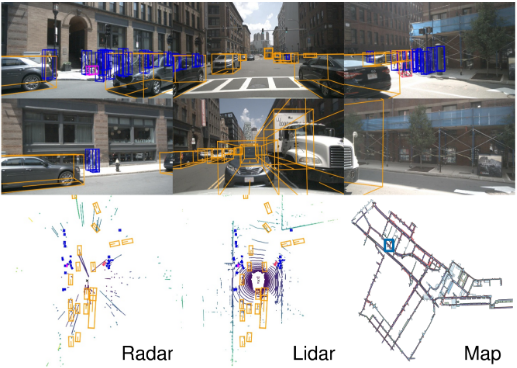
\includegraphics[width=\textwidth]{nuscenes_teaser.png}
\caption{A sample from the nuScenes dataset, showing the 6 camera views (top), along with Lidar and Radar point clouds (bottom left/middle) and the semantic map (bottom right). This full sensor suite provides a comprehensive view of the driving scene. (Image from \citep{caesar2020nuscenes})}
\label{fig:nuscenes_teaser}
\end{figure}

\begin{figure}[h]
\centering
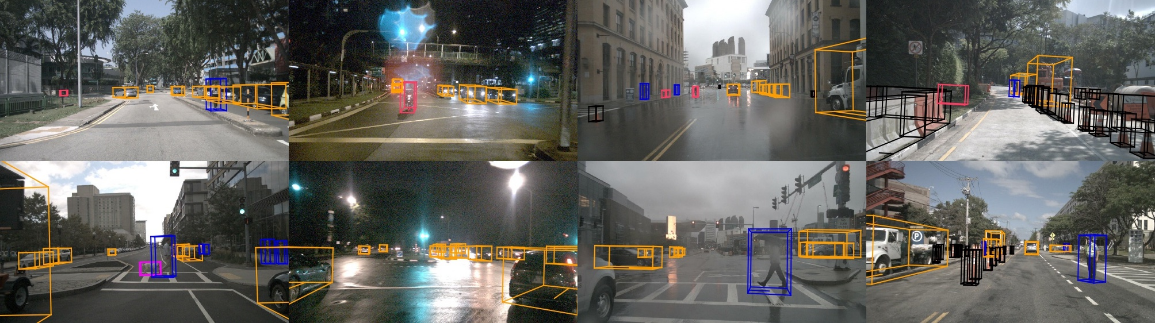
\includegraphics[width=\textwidth]{nuscenes_conditions.png}
\caption{Examples of the diverse conditions in nuScenes, including: (col 1) clear weather, (col 2) nighttime, (col 3) rain, and (col 4) construction zones. (Image from \citep{caesar2020nuscenes})}
\label{fig:nuscenes_conditions}
\end{figure}



% Chapter Template

\chapter{Methodology} % Main chapter title

\label{Chapter3} % Change X to a consecutive number; for referencing this chapter elsewhere, use \ref{ChapterX}

\lhead{Chapter 3. \emph{Methodology}} % Change X to a consecutive number; this is for the header on each page - perhaps a shortened title

%----------------------------------------------------------------------------------------
%\tSECTION 1
%---------------------------------------------------------------------------------------
\section{System Overview}

The core of this project is the integration of a powerful vision-based scene understanding model (BEVDepth) with a state-of-the-art motion forecasting model (AgentFormer). The hypothesis is that the rich, dense visual context provided by BEVDepth can enhance AgentFormer's ability to predict future trajectories of agents in a scene. This section details the architecture of the integrated system and the methodology used for its implementation.

Figure \ref{fig:system_overview} presents a high-level overview of the integrated model. The system consists of two main components: the BEVDepth model for feature extraction and the AgentFormer model for motion forecasting.

\begin{figure}[h]
\centering
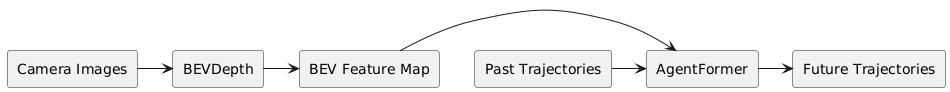
\includegraphics[width=0.8\textwidth]{system_overview.png}
\caption{High-level overview of the integrated BEVDepth and AgentFormer model.}
\label{fig:system_overview}
\end{figure}

The workflow is as follows:
\begin{enumerate}
    \item The BEVDepth model takes a sequence of camera images as input and generates a dense Bird's-Eye-View (BEV) feature map of the scene.
    \item The AgentFormer model takes the past trajectories of agents in the scene as input.
    \item The BEV feature map is then fused with the agent's trajectory information within the AgentFormer model.
    \item The fused representation is used by AgentFormer's transformer-based architecture to predict the future trajectories of the agents.
\end{enumerate}

The following sections provide a more detailed description of each component and the integration process.

\section{Experimental Setup}

The experiments for this thesis were conducted on a high-performance computing setup. The system was equipped with a 300GB solid-state drive (SSD) for fast data access, which is crucial for handling the large nuScenes dataset. For model training and inference, an NVIDIA RTX 5090 GPU with 32GB of VRAM was used. This powerful GPU enabled the training of deep learning models with large batch sizes and high-resolution inputs.

\section{Integration with AgentFormer}

The integration of the BEV features into the AgentFormer model is handled within the {\sloppy\texttt{AgentFormer/model/agentformer.py}} file. The core logic resides in the `AgentFormer` and `ContextEncoder` classes.

\subsection{AgentFormer Model}

The `AgentFormer` class's {\sloppy\texttt{\_\_init\_\_}} method checks for the {\sloppy\texttt{use\_bev}} flag in the configuration. If it is set to `True`, the following actions are taken:

\begin{enumerate}
    \item The `BaseLSSFPN` class from {\sloppy\texttt{model/bev/base\_lss\_fpn.py}} is imported and used to initialize the BEV encoder ({\sloppy\texttt{self.bev\_encoder}}).
    \item A fusion module, {\sloppy\texttt{self.bev\_fusion\_module}}, is created. This is a simple Multi-Layer Perceptron (MLP) designed to fuse the BEV features with the agent's trajectory features.
\end{enumerate}

In the `forward` pass of the `AgentFormer` model, the BEV features are either loaded from pre-computed files or extracted on-the-fly by the {\sloppy\texttt{bev\_encoder}}. These features are then passed to the `ContextEncoder`.

\subsection{Context Encoder}

The `ContextEncoder` is responsible for encoding the past trajectories of the agents. The integration of BEV features happens in its `forward` method.

\begin{enumerate}
    \item The method checks if a {\sloppy\texttt{bev\_feature\_map}} is available in the input data.
    \item If BEV features are present, the model samples features from the BEV map at the 2D location of each agent for each timestep in its past trajectory. This is achieved using the {\sloppy\texttt{grid\_sample}} function from PyTorch, which allows for differentiable sampling from a feature map.
    \item The sampled BEV features are then concatenated with the agent's existing trajectory features (e.g., position, velocity).
    \item The concatenated features are passed through the \texttt{bev\_fusion\_module} (the MLP) to produce a fused feature vector.
    \item This fused feature vector is then used as the input to the AgentFormer's transformer encoder, allowing the model to reason about the agent's future motion based on both its past trajectory and the surrounding visual context from the BEV map.
\end{enumerate}

This methodology allows for a tight integration of visual and trajectory information, with the goal of improving the accuracy of motion forecasting. The following chapter will present the results of this integration and analyze the reasons for the observed performance.

% Chapter Template

\chapter{Results and Discussion} % Main chapter title

\label{Chapter4} % Change X to a consecutive number; for referencing this chapter elsewhere, use \ref{ChapterX}

\lhead{Chapter 4. \emph{Results and Discussion}} % Change X to a consecutive number; this is for the header on each page - perhaps a shortened title

%----------------------------------------------------------------------------------------
%\t\tSECTION 1
%---------------------------------------------------------------------------------------
\section{Evaluation Metrics}

The performance of the vision-augmented AgentFormer was evaluated on the nuScenes dataset and compared against the baseline AgentFormer model. The standard metrics for motion forecasting, Average Displacement Error (ADE) and Final Displacement Error (FDE), were used for the evaluation.

\subsection{Average Displacement Error (ADE)}

Average Displacement Error (ADE) is a widely used metric for evaluating trajectory forecasting models. It measures the average L2 distance between the predicted trajectory and the ground truth trajectory over all predicted timesteps. For a predicted trajectory $\hat{Y} = (\hat{y}_1, \hat{y}_2, ..., \hat{y}_T)$ and a ground truth trajectory $Y = (y_1, y_2, ..., y_T)$, the ADE is calculated as:

\begin{equation}
ADE = \frac{1}{T} \sum_{t=1}^{T} ||\hat{y}_t - y_t||_2
\end{equation}

where $T$ is the prediction horizon and $||\cdot||_2$ denotes the L2 norm. A lower ADE value indicates a better forecasting performance.

\subsection{Final Displacement Error (FDE)}

Final Displacement Error (FDE) is another common metric for trajectory forecasting. It measures the L2 distance between the predicted final destination and the ground truth final destination at the end of the prediction horizon $T$. The FDE is calculated as:

\begin{equation}
FDE = ||\hat{y}_T - y_T||_2
\end{equation}

A lower FDE value indicates a better prediction of the agent's final position.

\section{Experiments}

This section details the experimental procedure for training and evaluating the baseline (vanilla) AgentFormer and the vision-augmented AgentFormer models.

\subsection{Vanilla AgentFormer}

The baseline AgentFormer model was trained and evaluated using the standard configuration provided in the original implementation. The model was trained on the nuScenes dataset using only the trajectory data. The following command was used to initiate the training process:

\begin{verbatim}
python train.py --cfg nuscenes\_5sample\_agentformer
\end{verbatim}

This command uses the \texttt{nuscenes\_5sample\_agentformer.yml} configuration file, which defines the model architecture, training parameters, and data paths for the vanilla AgentFormer.

\subsection{BEV-Augmented AgentFormer}

The vision-augmented AgentFormer model was trained using the pre-computed BEV features. The training process was initiated with the following command:

\begin{verbatim}
python train.py --cfg nuscenes\_5sample\_agentformer\_bev
\end{verbatim}

This command uses the \texttt{nuscenes\_5sample\_agentformer\_bev.yml} configuration file. This file is similar to the vanilla configuration but with the following key differences:

\begin{itemize}
    \item \texttt{use\_bev: true}: Enables the use of BEV features.
    \item \texttt{freeze\_bev\_encoder: true}: Freezes the BEV encoder weights.
    \item \texttt{use\_precomputed\_bev: true}: Instructs the data loader to load the pre-computed BEV features.
\end{itemize}

By using the pre-computed features, the training process is significantly accelerated as the model does not need to extract BEV features from the raw image data during training.

\section{Quantitative Results}

\begin{table}[h]
\centering
\caption{Performance comparison of baseline and vision-augmented AgentFormer.}
\label{tab:results}
\begin{tabular}{lcc}
\toprule
\textbf{Model} & \textbf{ADE} & \textbf{FDE} \\
\midrule
Baseline AgentFormer & 4.8110 & 9.5486 \\
Vision-Augmented AgentFormer & 5.1939 & 11.0132 \\
\bottomrule
\end{tabular}
\end{table}

As shown in Table \ref{tab:results}, the vision-augmented AgentFormer performed worse than the baseline model on both ADE and FDE metrics. This result is counter-intuitive, as the addition of visual information was expected to improve the model's performance. The following section provides a detailed analysis of the potential reasons for this performance degradation.

\subsection{Vanilla Model Training Loss}

Figure \ref{fig:loss_curves_vanilla} shows the training loss curves for the baseline AgentFormer model. The plots show the average loss per epoch for the total loss, KLD loss, reconstruction loss, and diversity loss.

\begin{figure}[h]
\centering
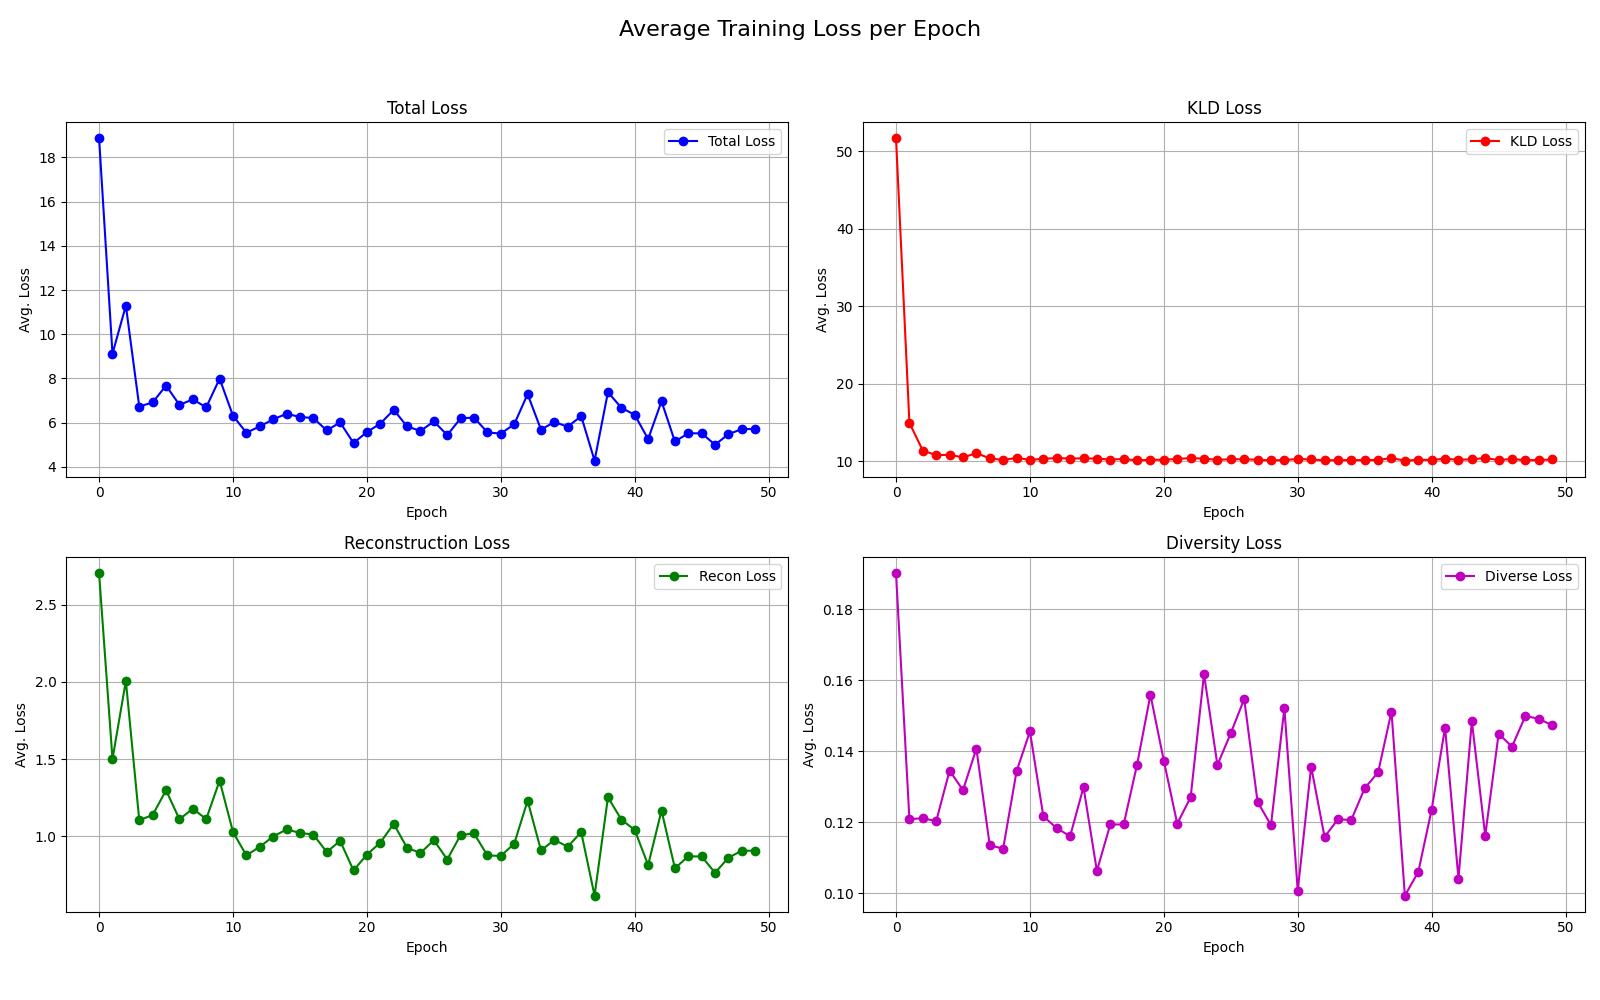
\includegraphics[width=\textwidth]{epoch_loss_curves_vanilla.png}
\caption{Average training loss per epoch for the baseline AgentFormer (Vanilla).}
\label{fig:loss_curves_vanilla}
\end{figure}

\subsection{BEV-Augmented Model Training Loss}

Figure \ref{fig:loss_curves_bev} shows the training loss curves for the vision-augmented AgentFormer model. The plots show the average loss per epoch for the total loss, KLD loss, MSE loss, and sample loss.

\begin{figure}[h]
\centering
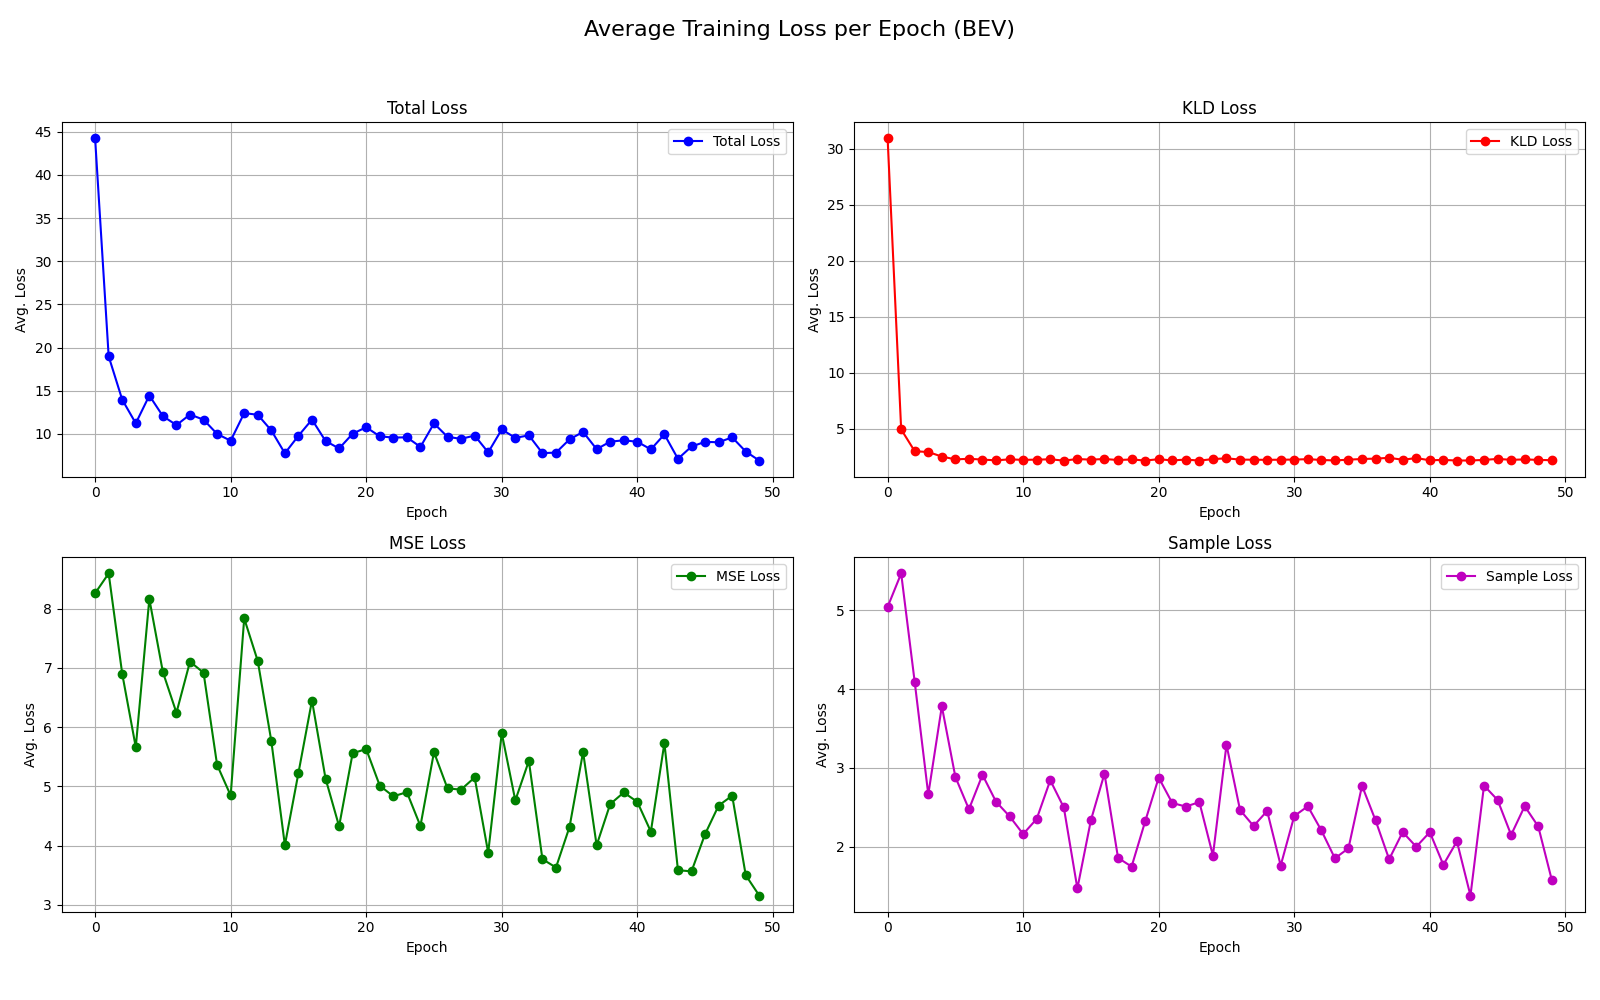
\includegraphics[width=\textwidth]{epoch_loss_curves_bev.png}
\caption{Average training loss per epoch for the vision-augmented AgentFormer (BEV).}
\label{fig:loss_curves_bev}
\end{figure}

\begin{itemize}
    \item \textbf{Total Loss:} The total loss is the sum of the other loss components. It shows a steep decrease in the first few epochs and then stabilizes, indicating that the model is learning. However, the final loss is still relatively high, which is consistent with the poor performance on the ADE and FDE metrics.
    \item \textbf{KLD Loss:} The Kullback-Leibler divergence (KLD) loss is part of the CVAE framework. It measures the difference between the learned latent distribution and the prior distribution. The KLD loss also shows a steep decrease in the beginning and then becomes stable. This indicates that the latent space is being learned correctly.
    \item \textbf{MSE Loss:} The Mean Squared Error (MSE) loss is the primary loss function for the trajectory prediction task. It measures the L2 distance between the predicted and ground truth trajectories. The MSE loss shows a decreasing trend, but with significant fluctuations. This volatility suggests that the model is struggling to find a stable solution. The high final value of the MSE loss is the main contributor to the high ADE and FDE scores.
    \item \textbf{Sample Loss:} The sample loss encourages the model to generate diverse samples. It also shows a decreasing trend with fluctuations, similar to the MSE loss.
\end{itemize}

The analysis of the loss curves provides further evidence for the suboptimal performance of the vision-augmented model. The instability in the MSE loss suggests that the model is not able to effectively integrate the visual information from the BEV features. The high variance in the loss indicates that for some training examples, the BEV features are helpful, while for others they are detrimental, leading to a high overall error. This is a strong indication that the fusion mechanism is not robust enough to handle the complexity of the multi-modal input.

\subsection{Comparative Analysis of Training Loss}

A comparison of the training loss curves for the vanilla and BEV-augmented models reveals a key difference in the training dynamics. While both models show a similar trend in the KLD and diversity/sample losses, the reconstruction/MSE loss behaves very differently.

The vanilla model's reconstruction loss shows a stable and consistent decrease, indicating that the model is effectively learning to reconstruct the ground truth trajectories. In contrast, the BEV-augmented model's MSE loss is highly volatile and fluctuates significantly throughout the training process. This suggests that the introduction of BEV features introduces a significant amount of noise and instability into the training process.

The higher and more unstable MSE loss of the BEV-augmented model is the primary reason for its worse performance compared to the vanilla model. The model is not able to effectively leverage the visual information from the BEV features and, in many cases, this information seems to be detrimental to the learning process. This further supports the hypothesis that a simple fusion mechanism is not sufficient to effectively combine the rich and dense BEV features with the sparse trajectory data.

\section{Analysis of Negative Results}

The unexpected negative results suggest that simply fusing BEV features with trajectory data is not sufficient to improve motion forecasting performance. This section explores several potential reasons for this outcome.

\subsection{Domain Mismatch}

The BEVDepth model was pre-trained on a large-scale dataset for 3D object detection. While this dataset is also from the autonomous driving domain, the distribution of scenes and the specific task it was trained on might be different from the motion forecasting task. This domain mismatch could lead to the BEV features not being optimally suited for trajectory prediction. The features that are important for object detection (e.g., precise object boundaries) might not be the most relevant for predicting future motion.

\subsection{Feature Incompatibility}

The BEV features are rich and dense, containing a vast amount of information about the scene. However, the AgentFormer model is primarily designed to work with sparse trajectory data. The simple fusion mechanism used in this project (concatenation followed by an MLP) might not be effective enough to bridge the gap between these two different modalities. The model might struggle to extract the relevant information from the dense BEV features and integrate it meaningfully with the trajectory information.

\subsection{Information Redundancy and Conflict}

The past trajectory of an agent already contains a significant amount of information about its future motion and the scene context (e.g., lane following behavior). The visual information from the BEV features might be redundant with this information. For example, if an agent is following a lane, its past trajectory already implies the lane geometry. The BEV features showing the same lane geometry might not add much new information. In the worst case, the visual information might even conflict with the trajectory information, leading to confusion and a decrease in performance.

\subsection{Sparsity of Relevant Information}

While the BEV map is dense, the information that is truly relevant for predicting the future motion of a specific agent might be very sparse. For example, the most important information might be the location of a traffic light, the presence of a pedestrian in a crosswalk, or the behavior of a single interacting vehicle. The model might struggle to identify these sparse but crucial pieces of information from the high-dimensional and noisy BEV feature map.

\subsection{Frozen BEV Encoder}

In this project, the BEV encoder was frozen to reduce the computational cost of training. This means that the BEV features were not fine-tuned for the motion forecasting task. The features that are optimal for object detection might not be optimal for trajectory prediction. Fine-tuning the BEV encoder on the motion forecasting task could allow it to learn features that are more relevant to the downstream task, potentially leading to better performance.

\subsection{Suboptimal Fusion Strategy}

The fusion strategy used in this project is a simple concatenation followed by an MLP. This is a common and straightforward approach, but it might not be the most effective way to fuse information from two different modalities. More sophisticated fusion techniques, such as cross-attention mechanisms, could be explored. Cross-attention would allow the model to selectively attend to the most relevant parts of the BEV feature map for each agent, potentially leading to a more effective fusion of information.

% Chapter Template

\chapter{Conclusion and Future Works} % Main chapter title

\label{Chapter5} % Change X to a consecutive number; for referencing this chapter elsewhere, use \ref{ChapterX}

\lhead{Chapter 5. \emph{Conclusion and Future Works}} % Change X to a consecutive number; this is for the header on each page - perhaps a shortened title

%----------------------------------------------------------------------------------------
%\t\tSECTION 1
%---------------------------------------------------------------------------------------
\section{Conclusion}

This thesis presented an investigation into the integration of Bird's-Eye-View (BEV) features from the BEVDepth model with the AgentFormer motion forecasting framework. The primary hypothesis was that the rich visual context provided by the BEV features would enhance the predictive accuracy of AgentFormer. However, the experimental results demonstrated a degradation in performance compared to the baseline AgentFormer model, which relies solely on trajectory data.

The detailed analysis of the methodology and the potential reasons for the negative results lead to a clear conclusion: simply \textit{plugging in} powerful, pre-trained visual features into a motion forecasting model does not guarantee performance improvement. The process of multi-modal fusion is complex and requires a careful and task-specific approach. The domain mismatch between the pre-training task of the visual model and the downstream forecasting task, the incompatibility of feature representations, and the suboptimal fusion strategy are all likely contributors to the observed negative results.

This work highlights the importance of a holistic approach to multi-modal fusion in the context of autonomous driving. It is not enough to simply combine state-of-the-art models from different domains. Instead, the fusion process itself must be a central part of the model design, and the features from each modality must be carefully adapted and integrated to be beneficial for the end task.

\section{Future Works}

The surprising results of this thesis open up several avenues for future research. The following are some promising directions that could lead to a more successful integration of visual information into motion forecasting models:

\subsection{Fine-tuning the BEV Encoder}

One of the major limitations of this work was the use of a frozen BEV encoder. Fine-tuning the BEV encoder on the motion forecasting task could allow it to learn visual features that are more relevant to trajectory prediction. This would help to bridge the domain gap between the object detection task on which BEVDepth was pre-trained and the motion forecasting task.

\subsection{Advanced Fusion Mechanisms}

The simple MLP-based fusion mechanism used in this project might not be sufficient to effectively combine the visual and trajectory information. Future work should explore more advanced fusion techniques, such as attention-based mechanisms. Cross-attention could enable the model to selectively focus on the most relevant parts of the BEV feature map for each agent, leading to a more context-aware and effective fusion.

\subsection{Targeted Visual Representations}

Instead of using the entire dense BEV feature map, future research could focus on identifying and extracting the most relevant visual features for motion forecasting. This could involve designing a more compact and targeted visual representation that only includes information about key scene elements, such as lane geometry, traffic lights, and crosswalks. This would reduce the dimensionality of the visual input and make it easier for the model to extract the relevant signals.

\subsection{End-to-End Training}

Ultimately, the most promising approach would be to train the entire system end-to-end. This would allow the visual and motion forecasting components of the model to learn and adapt to each other, leading to a more synergistic and effective integration. While computationally expensive, end-to-end training would allow the model to learn the optimal visual features and fusion strategy for the specific task of motion forecasting.

By exploring these future research directions, we can move closer to developing motion forecasting models that can effectively leverage the rich information available in the visual world, leading to safer and more reliable autonomous driving systems.

%% Chapter Template

\chapter{Results and Discussion} % Main chapter title

\label{Chapter4} % Change X to a consecutive number; for referencing this chapter elsewhere, use \ref{ChapterX}

\lhead{Chapter 4. \emph{Results and Discussion}} % Change X to a consecutive number; this is for the header on each page - perhaps a shortened title

%----------------------------------------------------------------------------------------
%\t\tSECTION 1
%---------------------------------------------------------------------------------------
\section{Evaluation Metrics}

The performance of the vision-augmented AgentFormer was evaluated on the nuScenes dataset and compared against the baseline AgentFormer model. The standard metrics for motion forecasting, Average Displacement Error (ADE) and Final Displacement Error (FDE), were used for the evaluation.

\subsection{Average Displacement Error (ADE)}

Average Displacement Error (ADE) is a widely used metric for evaluating trajectory forecasting models. It measures the average L2 distance between the predicted trajectory and the ground truth trajectory over all predicted timesteps. For a predicted trajectory $\hat{Y} = (\hat{y}_1, \hat{y}_2, ..., \hat{y}_T)$ and a ground truth trajectory $Y = (y_1, y_2, ..., y_T)$, the ADE is calculated as:

\begin{equation}
ADE = \frac{1}{T} \sum_{t=1}^{T} ||\hat{y}_t - y_t||_2
\end{equation}

where $T$ is the prediction horizon and $||\cdot||_2$ denotes the L2 norm. A lower ADE value indicates a better forecasting performance.

\subsection{Final Displacement Error (FDE)}

Final Displacement Error (FDE) is another common metric for trajectory forecasting. It measures the L2 distance between the predicted final destination and the ground truth final destination at the end of the prediction horizon $T$. The FDE is calculated as:

\begin{equation}
FDE = ||\hat{y}_T - y_T||_2
\end{equation}

A lower FDE value indicates a better prediction of the agent's final position.

\section{Experiments}

This section details the experimental procedure for training and evaluating the baseline (vanilla) AgentFormer and the vision-augmented AgentFormer models.

\subsection{Vanilla AgentFormer}

The baseline AgentFormer model was trained and evaluated using the standard configuration provided in the original implementation. The model was trained on the nuScenes dataset using only the trajectory data. The following command was used to initiate the training process:

\begin{verbatim}
python train.py --cfg nuscenes\_5sample\_agentformer
\end{verbatim}

This command uses the \texttt{nuscenes\_5sample\_agentformer.yml} configuration file, which defines the model architecture, training parameters, and data paths for the vanilla AgentFormer.

\subsection{BEV-Augmented AgentFormer}

The vision-augmented AgentFormer model was trained using the pre-computed BEV features. The training process was initiated with the following command:

\begin{verbatim}
python train.py --cfg nuscenes\_5sample\_agentformer\_bev
\end{verbatim}

This command uses the \texttt{nuscenes\_5sample\_agentformer\_bev.yml} configuration file. This file is similar to the vanilla configuration but with the following key differences:

\begin{itemize}
    \item \texttt{use\_bev: true}: Enables the use of BEV features.
    \item \texttt{freeze\_bev\_encoder: true}: Freezes the BEV encoder weights.
    \item \texttt{use\_precomputed\_bev: true}: Instructs the data loader to load the pre-computed BEV features.
\end{itemize}

By using the pre-computed features, the training process is significantly accelerated as the model does not need to extract BEV features from the raw image data during training.

\section{Quantitative Results}

\begin{table}[h]
\centering
\caption{Performance comparison of baseline and vision-augmented AgentFormer.}
\label{tab:results}
\begin{tabular}{lcc}
\toprule
\textbf{Model} & \textbf{ADE} & \textbf{FDE} \\
\midrule
Baseline AgentFormer & 4.8110 & 9.5486 \\
Vision-Augmented AgentFormer & 5.1939 & 11.0132 \\
\bottomrule
\end{tabular}
\end{table}

As shown in Table \ref{tab:results}, the vision-augmented AgentFormer performed worse than the baseline model on both ADE and FDE metrics. This result is counter-intuitive, as the addition of visual information was expected to improve the model's performance. The following section provides a detailed analysis of the potential reasons for this performance degradation.

\subsection{Vanilla Model Training Loss}

Figure \ref{fig:loss_curves_vanilla} shows the training loss curves for the baseline AgentFormer model. The plots show the average loss per epoch for the total loss, KLD loss, reconstruction loss, and diversity loss.

\begin{figure}[h]
\centering
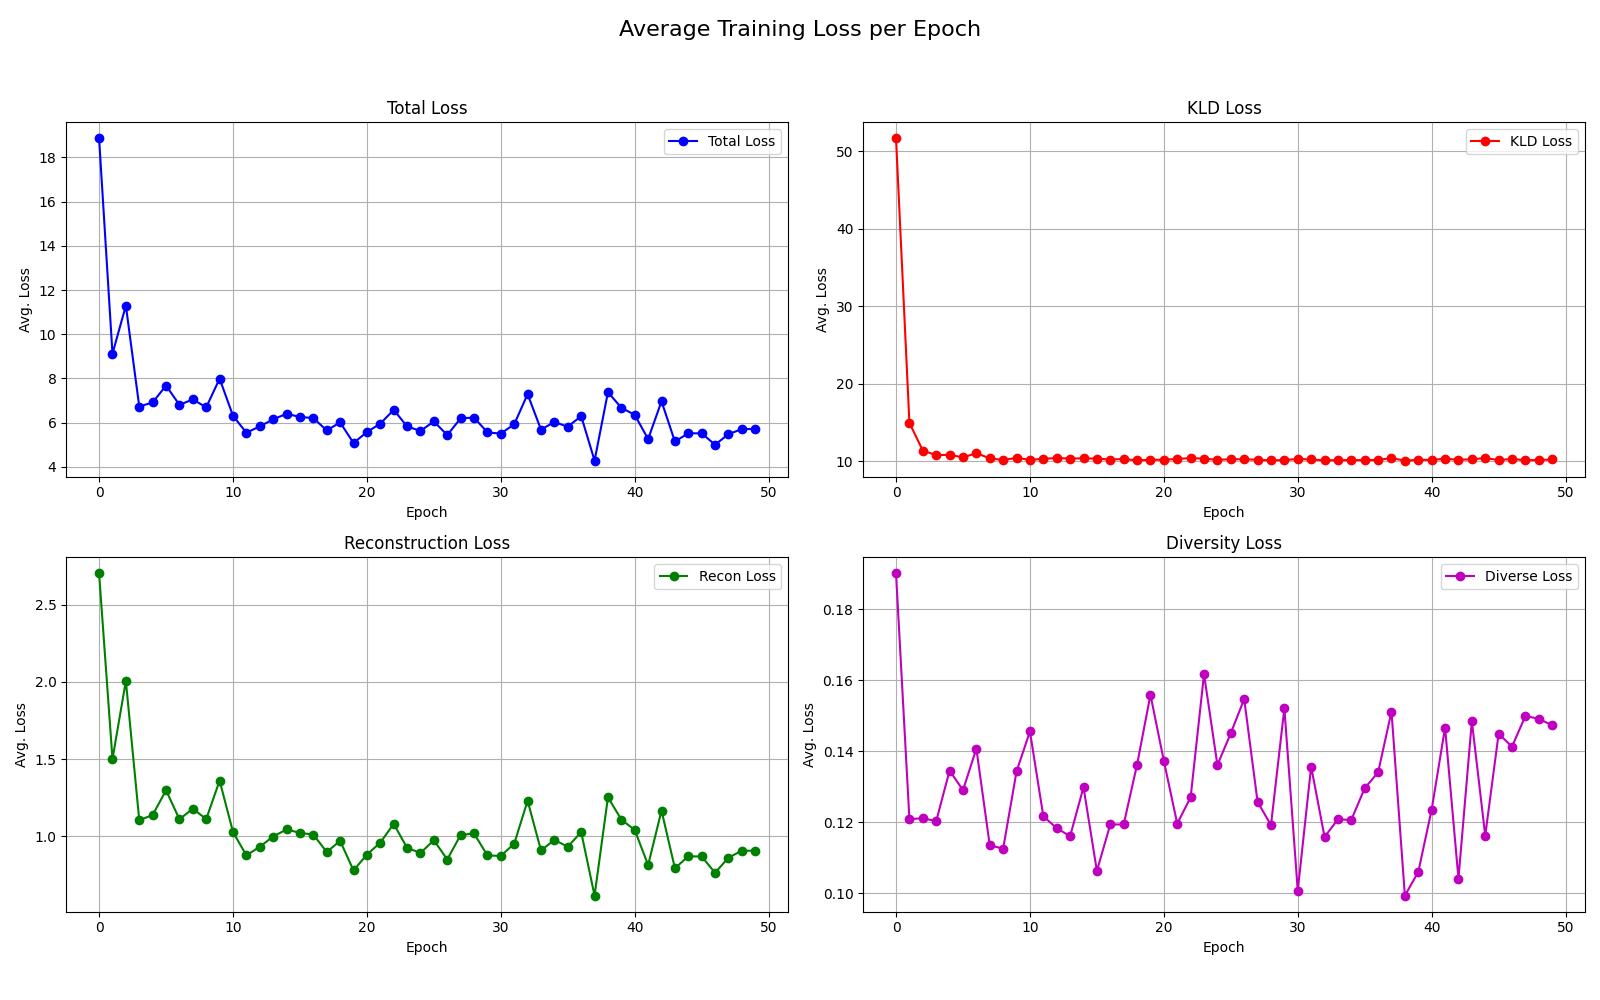
\includegraphics[width=\textwidth]{epoch_loss_curves_vanilla.png}
\caption{Average training loss per epoch for the baseline AgentFormer (Vanilla).}
\label{fig:loss_curves_vanilla}
\end{figure}

\subsection{BEV-Augmented Model Training Loss}

Figure \ref{fig:loss_curves_bev} shows the training loss curves for the vision-augmented AgentFormer model. The plots show the average loss per epoch for the total loss, KLD loss, MSE loss, and sample loss.

\begin{figure}[h]
\centering
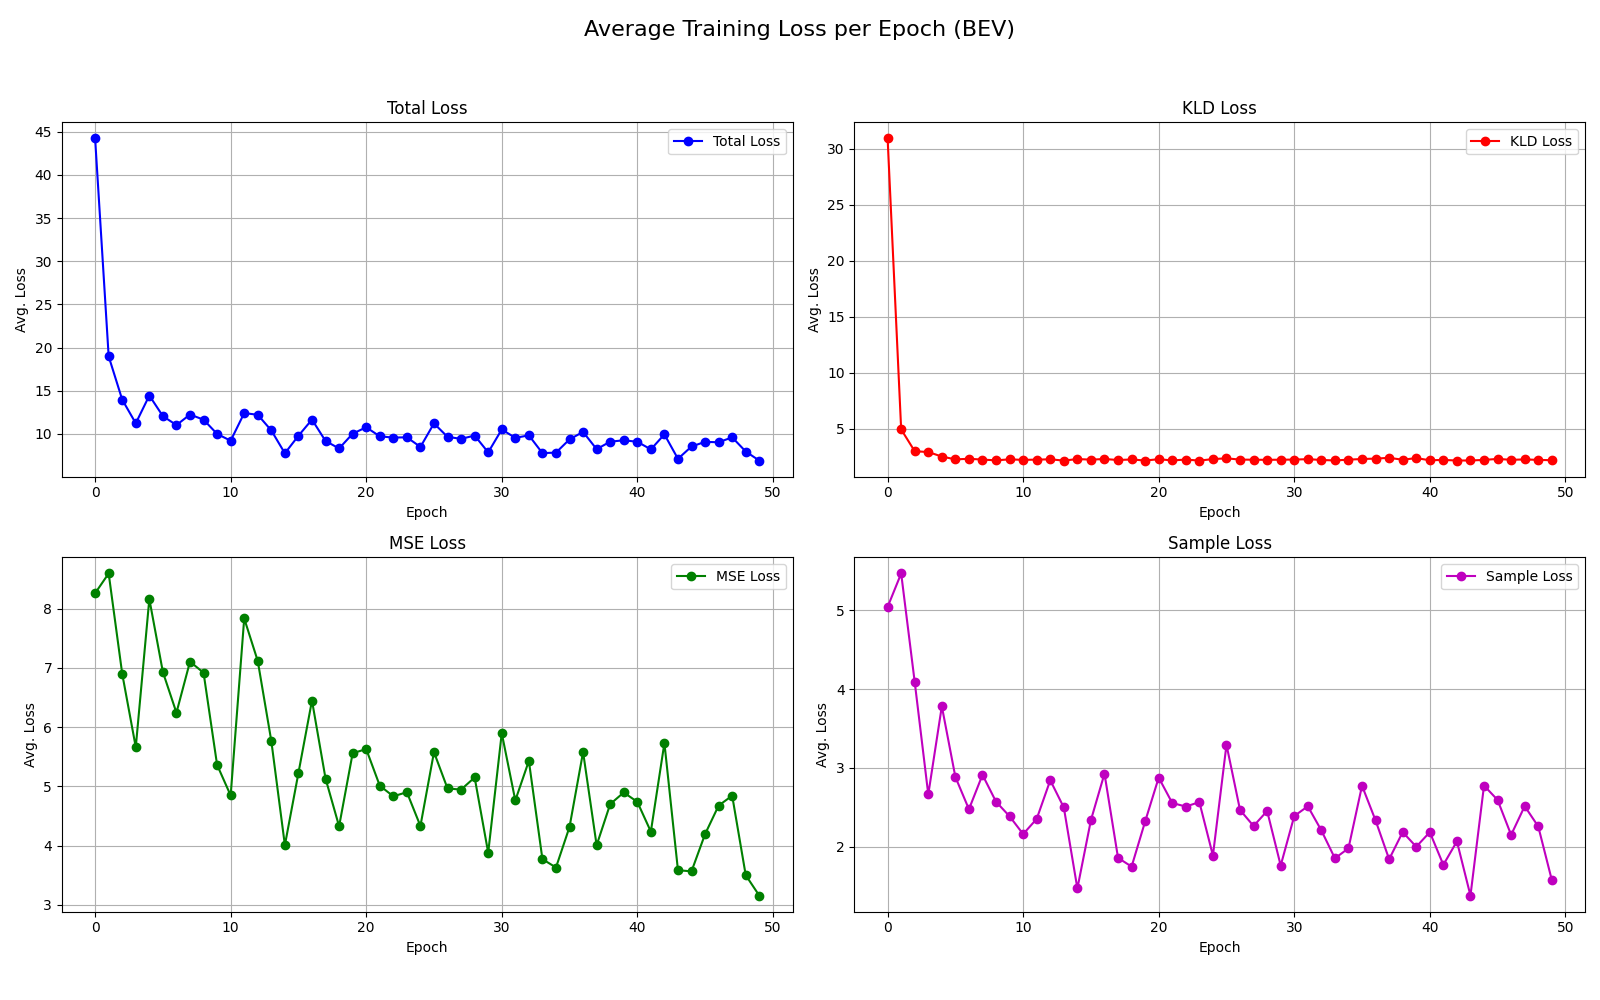
\includegraphics[width=\textwidth]{epoch_loss_curves_bev.png}
\caption{Average training loss per epoch for the vision-augmented AgentFormer (BEV).}
\label{fig:loss_curves_bev}
\end{figure}

\begin{itemize}
    \item \textbf{Total Loss:} The total loss is the sum of the other loss components. It shows a steep decrease in the first few epochs and then stabilizes, indicating that the model is learning. However, the final loss is still relatively high, which is consistent with the poor performance on the ADE and FDE metrics.
    \item \textbf{KLD Loss:} The Kullback-Leibler divergence (KLD) loss is part of the CVAE framework. It measures the difference between the learned latent distribution and the prior distribution. The KLD loss also shows a steep decrease in the beginning and then becomes stable. This indicates that the latent space is being learned correctly.
    \item \textbf{MSE Loss:} The Mean Squared Error (MSE) loss is the primary loss function for the trajectory prediction task. It measures the L2 distance between the predicted and ground truth trajectories. The MSE loss shows a decreasing trend, but with significant fluctuations. This volatility suggests that the model is struggling to find a stable solution. The high final value of the MSE loss is the main contributor to the high ADE and FDE scores.
    \item \textbf{Sample Loss:} The sample loss encourages the model to generate diverse samples. It also shows a decreasing trend with fluctuations, similar to the MSE loss.
\end{itemize}

The analysis of the loss curves provides further evidence for the suboptimal performance of the vision-augmented model. The instability in the MSE loss suggests that the model is not able to effectively integrate the visual information from the BEV features. The high variance in the loss indicates that for some training examples, the BEV features are helpful, while for others they are detrimental, leading to a high overall error. This is a strong indication that the fusion mechanism is not robust enough to handle the complexity of the multi-modal input.

\subsection{Comparative Analysis of Training Loss}

A comparison of the training loss curves for the vanilla and BEV-augmented models reveals a key difference in the training dynamics. While both models show a similar trend in the KLD and diversity/sample losses, the reconstruction/MSE loss behaves very differently.

The vanilla model's reconstruction loss shows a stable and consistent decrease, indicating that the model is effectively learning to reconstruct the ground truth trajectories. In contrast, the BEV-augmented model's MSE loss is highly volatile and fluctuates significantly throughout the training process. This suggests that the introduction of BEV features introduces a significant amount of noise and instability into the training process.

The higher and more unstable MSE loss of the BEV-augmented model is the primary reason for its worse performance compared to the vanilla model. The model is not able to effectively leverage the visual information from the BEV features and, in many cases, this information seems to be detrimental to the learning process. This further supports the hypothesis that a simple fusion mechanism is not sufficient to effectively combine the rich and dense BEV features with the sparse trajectory data.

\section{Analysis of Negative Results}

The unexpected negative results suggest that simply fusing BEV features with trajectory data is not sufficient to improve motion forecasting performance. This section explores several potential reasons for this outcome.

\subsection{Domain Mismatch}

The BEVDepth model was pre-trained on a large-scale dataset for 3D object detection. While this dataset is also from the autonomous driving domain, the distribution of scenes and the specific task it was trained on might be different from the motion forecasting task. This domain mismatch could lead to the BEV features not being optimally suited for trajectory prediction. The features that are important for object detection (e.g., precise object boundaries) might not be the most relevant for predicting future motion.

\subsection{Feature Incompatibility}

The BEV features are rich and dense, containing a vast amount of information about the scene. However, the AgentFormer model is primarily designed to work with sparse trajectory data. The simple fusion mechanism used in this project (concatenation followed by an MLP) might not be effective enough to bridge the gap between these two different modalities. The model might struggle to extract the relevant information from the dense BEV features and integrate it meaningfully with the trajectory information.

\subsection{Information Redundancy and Conflict}

The past trajectory of an agent already contains a significant amount of information about its future motion and the scene context (e.g., lane following behavior). The visual information from the BEV features might be redundant with this information. For example, if an agent is following a lane, its past trajectory already implies the lane geometry. The BEV features showing the same lane geometry might not add much new information. In the worst case, the visual information might even conflict with the trajectory information, leading to confusion and a decrease in performance.

\subsection{Sparsity of Relevant Information}

While the BEV map is dense, the information that is truly relevant for predicting the future motion of a specific agent might be very sparse. For example, the most important information might be the location of a traffic light, the presence of a pedestrian in a crosswalk, or the behavior of a single interacting vehicle. The model might struggle to identify these sparse but crucial pieces of information from the high-dimensional and noisy BEV feature map.

\subsection{Frozen BEV Encoder}

In this project, the BEV encoder was frozen to reduce the computational cost of training. This means that the BEV features were not fine-tuned for the motion forecasting task. The features that are optimal for object detection might not be optimal for trajectory prediction. Fine-tuning the BEV encoder on the motion forecasting task could allow it to learn features that are more relevant to the downstream task, potentially leading to better performance.

\subsection{Suboptimal Fusion Strategy}

The fusion strategy used in this project is a simple concatenation followed by an MLP. This is a common and straightforward approach, but it might not be the most effective way to fuse information from two different modalities. More sophisticated fusion techniques, such as cross-attention mechanisms, could be explored. Cross-attention would allow the model to selectively attend to the most relevant parts of the BEV feature map for each agent, potentially leading to a more effective fusion of information.
 
%% Chapter Template

\chapter{Conclusion and Future Works} % Main chapter title

\label{Chapter5} % Change X to a consecutive number; for referencing this chapter elsewhere, use \ref{ChapterX}

\lhead{Chapter 5. \emph{Conclusion and Future Works}} % Change X to a consecutive number; this is for the header on each page - perhaps a shortened title

%----------------------------------------------------------------------------------------
%\t\tSECTION 1
%---------------------------------------------------------------------------------------
\section{Conclusion}

This thesis presented an investigation into the integration of Bird's-Eye-View (BEV) features from the BEVDepth model with the AgentFormer motion forecasting framework. The primary hypothesis was that the rich visual context provided by the BEV features would enhance the predictive accuracy of AgentFormer. However, the experimental results demonstrated a degradation in performance compared to the baseline AgentFormer model, which relies solely on trajectory data.

The detailed analysis of the methodology and the potential reasons for the negative results lead to a clear conclusion: simply \textit{plugging in} powerful, pre-trained visual features into a motion forecasting model does not guarantee performance improvement. The process of multi-modal fusion is complex and requires a careful and task-specific approach. The domain mismatch between the pre-training task of the visual model and the downstream forecasting task, the incompatibility of feature representations, and the suboptimal fusion strategy are all likely contributors to the observed negative results.

This work highlights the importance of a holistic approach to multi-modal fusion in the context of autonomous driving. It is not enough to simply combine state-of-the-art models from different domains. Instead, the fusion process itself must be a central part of the model design, and the features from each modality must be carefully adapted and integrated to be beneficial for the end task.

\section{Future Works}

The surprising results of this thesis open up several avenues for future research. The following are some promising directions that could lead to a more successful integration of visual information into motion forecasting models:

\subsection{Fine-tuning the BEV Encoder}

One of the major limitations of this work was the use of a frozen BEV encoder. Fine-tuning the BEV encoder on the motion forecasting task could allow it to learn visual features that are more relevant to trajectory prediction. This would help to bridge the domain gap between the object detection task on which BEVDepth was pre-trained and the motion forecasting task.

\subsection{Advanced Fusion Mechanisms}

The simple MLP-based fusion mechanism used in this project might not be sufficient to effectively combine the visual and trajectory information. Future work should explore more advanced fusion techniques, such as attention-based mechanisms. Cross-attention could enable the model to selectively focus on the most relevant parts of the BEV feature map for each agent, leading to a more context-aware and effective fusion.

\subsection{Targeted Visual Representations}

Instead of using the entire dense BEV feature map, future research could focus on identifying and extracting the most relevant visual features for motion forecasting. This could involve designing a more compact and targeted visual representation that only includes information about key scene elements, such as lane geometry, traffic lights, and crosswalks. This would reduce the dimensionality of the visual input and make it easier for the model to extract the relevant signals.

\subsection{End-to-End Training}

Ultimately, the most promising approach would be to train the entire system end-to-end. This would allow the visual and motion forecasting components of the model to learn and adapt to each other, leading to a more synergistic and effective integration. While computationally expensive, end-to-end training would allow the model to learn the optimal visual features and fusion strategy for the specific task of motion forecasting.

By exploring these future research directions, we can move closer to developing motion forecasting models that can effectively leverage the rich information available in the visual world, leading to safer and more reliable autonomous driving systems.
 
%\input{Chapters/Chapter6} 
%\input{Chapters/Chapter7} 

%----------------------------------------------------------------------------------------
%\tTHESIS CONTENT - APPENDICES
%----------------------------------------------------------------------------------------

\addtocontents{toc}{\vspace{2em}} % Add a gap in the Contents, for aesthetics

\appendix % Cue to tell LaTeX that the following 'chapters' are Appendices

% Include the appendices of the thesis as separate files from the Appendices folder
% Uncomment the lines as you write the Appendices

%\input{Appendices/AppendixA}
%\input{Appendices/AppendixB}
%\input{Appendices/AppendixC}

\addtocontents{toc}{} % Add a gap in the Contents, for aesthetics

\backmatter

%----------------------------------------------------------------------------------------
%\tBIBLIOGRAPHY
%----------------------------------------------------------------------------------------
%\nocite{*}
\label{Bibliography}

\lhead{\emph{Bibliography}} % Change the page header to say "Bibliography"

\bibliographystyle{apalike} % Use the "custom" BibTeX style for formatting the Bibliography


\bibliography{Bibliography} % The references (bibliography) information are stored in the file named "Bibliography.bib"

\end{document}  
